\documentclass{beamer}

\usepackage{tikz}
\usetikzlibrary{positioning,matrix, arrows.meta}
\usepackage{color}
\newcommand{\vet}[1]{\foreach \num in {#1}{\el{\num}}}
\newcommand{\vetempty}[1]{\foreach \num in {#1}{\elempty{\num}}}
\newcommand{\el}[1]{\tikz{\node[font=\huge, minimum size=1cm, draw]{#1}}}
\newcommand{\elempty}[1]{\tikz{\node[font=\small, minimum size=1cm, draw=white, fill=white]{#1}}}
\newcommand{\bl}{\color{blue}}
\newcommand{\gr}{\color{gray}}
\newcommand{\re}{\color{red}}
\newcommand{\tcb}[1]{\textcolor{blue}{#1}}
\newcommand{\tcg}[1]{\textcolor{green}{#1}}
\newcommand{\tcr}[1]{\textcolor{red}{#1}}
\newcommand{\ar}{\tikz{\draw [->] (0,0) -- (0,0.4)}}
\newcommand{\nd}{\color{white!0}.}

\usepackage{beamerthemeSingapore}
\usepackage{graphicx}
%\usepackage{here}
\usepackage{url}
\usepackage[brazil]{babel}
\usepackage[T1]{fontenc}
\usepackage[utf8]{inputenc}
\usepackage[tight,raggedright]{subfigure}
\usepackage[alf]{abntex2cite}
\usepackage{listings}
\usepackage{minted}
\usepackage{algorithm2e}
\usepackage{amsmath}
\usepackage{pdfpages}
% Please add the following required packages to your document preamble:
\usepackage{booktabs}
\usepackage{ragged2e}
\usepackage{etoolbox}
\usepackage{mathtools}
\DeclarePairedDelimiter{\ceil}{\lceil}{\rceil}

\apptocmd{\frame}{}{\justifying}{} % Allow optional arguments after frame.

% TODO TODO TODO TODO TODO TODO TODO
\title{05 - Mergesort}
\author{Prof. Alex Kutzke}
\date{Maio de 2021}

\begin{document}

	% ==========================================
	\begin{frame}
		\begin{center}
			% TODO TODO TODO TODO TODO TODO
			\large{Setor de Educação Profissional e Tecnológica}\\
			Tecnologia em Análise e Desenvolvimento de Sistemas\\
			\vspace{1cm}			
			\small{DS141 - Estruturas de Dados II}
		\end{center}
		\titlepage
		\begin{center}
			Slides adaptados do material produzido\\pelo Prof. Reinaldo Fortes
		\end{center}
	\end{frame}
	% ==========================================

	% ==========================================
	\begin{frame}[c]{Roteiro}
		\tableofcontents

	\end{frame}
	% ==========================================

	\section{Introdução}

	\begin{frame}[c]{Motivação}
		\begin{itemize}
			\item É preciso resolver um problema com uma entrada grande;
			\item Para facilitar a resolução do problema, a entrada é quebrada em pedaços menores (divisão);
			\item Cada pedaço da entrada é então tratado separadamente (conquista);
			\item Ao final, os resultados parciais são combinados para gerar o resultado final procurado.
		\end{itemize}
	\end{frame}

	\begin{frame}[c]{Motivação}
		A técnica de \textbf{divisão e conquista} consiste de \textbf{3 passos}:
		\begin{description}
			\justifying
			\item[Divisão]: dividir o problema original em subproblemas menores;
			\item[Conquista]: resolver cada subproblema (talvez recursivamente);
			\item[Combinação]: combinar as soluções encontradas, compondo uma solução para o problema original.
		\end{description}
	\end{frame}

	\begin{frame}[c]{A técnica}
		\begin{itemize}
			\item Algoritmos baseados em divisão e conquista são, em geral, \tcr{recursivos} (mas não necessariamente);
			\item A maioria dos algoritmos de divisão e conquista divide o problema em subproblemas da mesma natureza, de tamanho $\displaystyle \frac{n}{b}$;
			\item Vantagens:
			\begin{itemize}
				\item \textbf{Uso eficiente da memória cache}: ao final da fase de divisão grande parte dos dados necessários para a fase de combinação já estão disponíveis na cache:
				\begin{itemize}
					\item Com isso, requerem um número menor de acessos à memória (lembram de S.O.)?
				\end{itemize}
			\item \textbf{São altamente paralelizáveis}: se existirem vários processadores disponíveis, a estratégia propiciará eficiência;
			\end{itemize}
		\end{itemize}
	\end{frame}

	\begin{frame}[c]{Quando utilizar?}
		Existem três condições que indicam que a estratégia de divisão e conquista pode ser utilizada com sucesso:
		\begin{itemize}
			\justifying
			\item Deve ser possível decompor uma instância em sub-instâncias;
			\item A combinação dos resultados deve ser eficiente (trivial, se possível);
			\item As sub-instâncias devem ser mais ou menos do mesmo tamanho.
		\end{itemize}
	\end{frame}

	\begin{frame}[c,fragile]{Algoritmo genérico}
		\begin{algorithm}[H]
			\small
			\SetKwFunction{FDivisao}{divisao\_e\_conquista}
	    \SetKwProg{Fn}{Function}{:}{}
			\Fn{\FDivisao{x}}{
				\eIf {x pequeno ou simples}{
					\textbf{return} $x$
				}
				{
					decompor $x$ em $n$ conjuntos menores: $x[0], x[1], \ldots, x[n-1]$\\
					\For{$i$ in $[0, 1, \ldots, n-1]$}{
						$y[i] = divisao\_e\_conquista(x[i])$
					}
					combinar $y[0], y[1], \ldots, y[n-1]$ em $y$\\
					\textbf{return} $y$
				}

			}
		\end{algorithm}
	\end{frame}

	\begin{frame}[c]{Utilização na ordenação}
		\begin{itemize}
			\item Métodos de ordenação que utilizam-se da \textbf{Divisão e Conquista}:
			\begin{itemize}
				\item Mergesort, Quicksort e vários outros;
			\end{itemize}
			\item Principal diferença entre Mergesort e Quicksort:
			\begin{itemize}
				\item \textbf{Mergesort}: sempre divide o problema de forma balanceada (subproblemas de mesmo tamanho);
				\item \textbf{Quicksort}: utiliza o conceito de \tcb{pivô} para dividir o problema em subproblemas (subproblemas de tamanhos diferentes);
			\end{itemize}
		\end{itemize}
	\end{frame}

	\section{Mergesort}

	\begin{frame}[c]{Algoritmo}
		\begin{enumerate}
			\item Divida a coleção em duas partes;
			\item Ordene as duas partes utilizando o mesmo Algoritmo;
			\item Intercale (merge) as duas partes ordenadas, obtendo uma coleção ordenada.
		\end{enumerate}
	\end{frame}

	\begin{frame}[c]{Funcionamento}
		A execução do \textbf{Mergesort} pode ser facilmente descrita por uma espécie de árvore (binária):
		\begin{itemize}
			\item Cada nó representa uma chamada recursiva do \textbf{Mergesort};
			\item O nó raiz é a chamada inicial;
			\item Os nós folha são vetores de 1 ou 2 números (caso base).
		\end{itemize}
	  \begin{figure}[h]
	  	\centering
	  	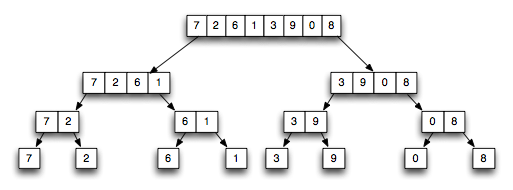
\includegraphics[width=10cm]{img/merge-tree.png}
			\caption{Exemplo divisões mergesort. Fonte: \url{http://www.codenlearn.com/2011/10/simple-merge-sort.html}}
	  \end{figure}
	\end{frame}

	% ==========================================
	\begin{frame}[c]{Execução}
		\begin{center}
			Utilize o Mergesort para ordenar a seguinte coleção de números:
			\vetempty{0,1,2,3,4,5,6}\\
			\vet{38,27,43,3,9,82,10}\\
		\end{center}
	\end{frame}
	% ==========================================
	
	\begin{frame}[c]{Execução}
	  \begin{figure}[h]
	  	\centering
	  	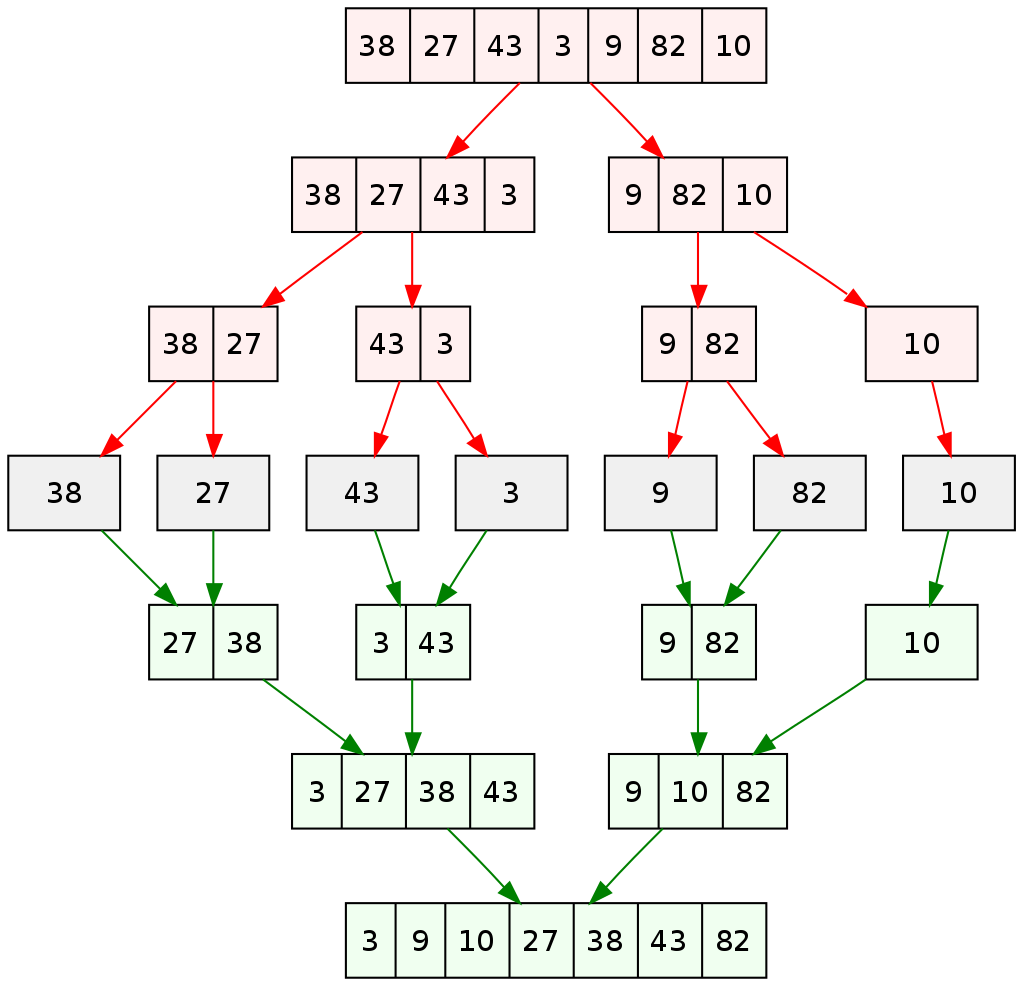
\includegraphics[width=7cm]{img/merge-wiki.png}
			\caption{\small Exemplo execução mergesort. Fonte: \url{https://en.wikipedia.org/wiki/Merge_sort}}
	  \end{figure}
	\end{frame}
	% ==========================================

	\begin{frame}[c]{Ordem de Complexidade}
		\begin{enumerate}
			\item Similar a Busca Binária;
			\item A altura \textbf{$h$} da árvore de execução é \textbf{$\log_{2}{n}$};
			\item A quantidade de operações em cada nível da árvore é, assintoticamente, \textbf{$O(n)$};
			\item Logo: Mergesort tem uma complexidade de \textbf{$O(n \log_{2}{n})$}.
		\end{enumerate}
	  \begin{figure}[h]
	  	\centering
	  	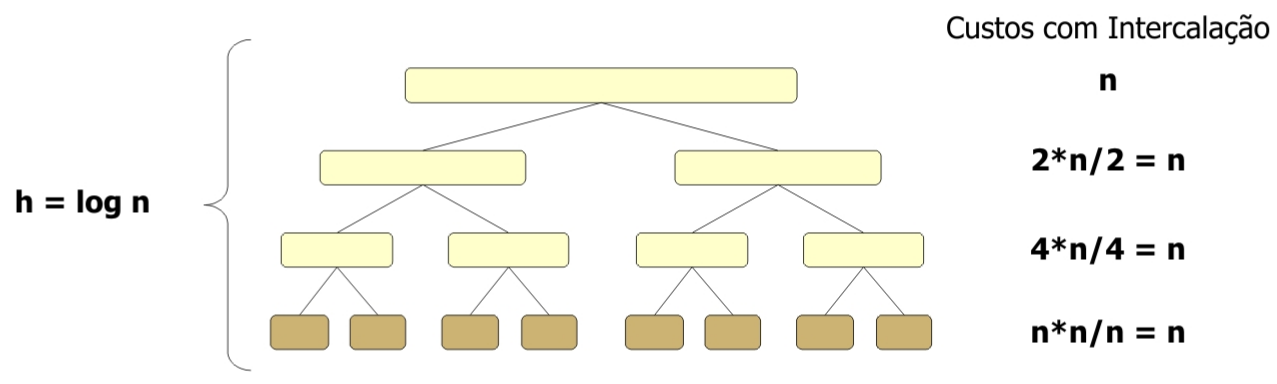
\includegraphics[width=\textwidth]{img/merge-tren-analysis.png}
			\caption{\small Análise de árvore de execução do mergesort. Fonte: Slides do Prof. Reinaldo Fortes (\url{http://www.decom.ufop.br/reifortes})}.
	  \end{figure}
	\end{frame}

	\section{Implementação Recursiva}

	\begin{frame}[fragile]{Mergesort Recursivo}

		\begin{minted}[
				frame=lines,
				framesep=2mm,
				baselinestretch=1.2,
				fontsize=\footnotesize,
				linenos
			]{c}
void mergeSort(int *v, int n) {
	mergeSort_ordena (v, 0, n-1);
}

void mergeSort_ordena (int *v, int esq , int dir) {
	if (esq == dir)
		return;

	int meio = (esq + dir) / 2;
	mergeSort_ordena (v, esq , meio);
	mergeSort_ordena (v, meio+1, dir);
	merge (v, esq , meio , dir);
}
		\end{minted}
	\end{frame}
	
	\begin{frame}[fragile]{Merge}

		\begin{minted}[
				frame=lines,
				framesep=2mm,
				baselinestretch=1.2,
				fontsize=\footnotesize,
				linenos
			]{c}
void merge(int * a, int l, int m, int r)
{
  int i,j,k, *aux;
  aux = (int *) malloc(sizeof(int) * r+1);

  for(i=m+1; i > l; i--) aux[i-1] = a[i-1];
  for(j=m; j < r; j++) aux[r+m-j] = a[j+1];

  for(k=l; k<=r; k++)
    if(aux[j] < aux[i]) a[k] = aux[j--];
    else                a[k] = aux[i++];
}
		\end{minted}
	\end{frame}
	
	% ==========================================
	\begin{frame}
		\frametitle{Análise empírica}

		Estimativas:
		\begin{itemize}
				\item Laptop executa $10^8$ comparações por segundo;
				\item Supercomputador executa $10^{12}$ comparações por segundo;
		\end{itemize}

	  \begin{figure}[h]
	  	\centering
	  	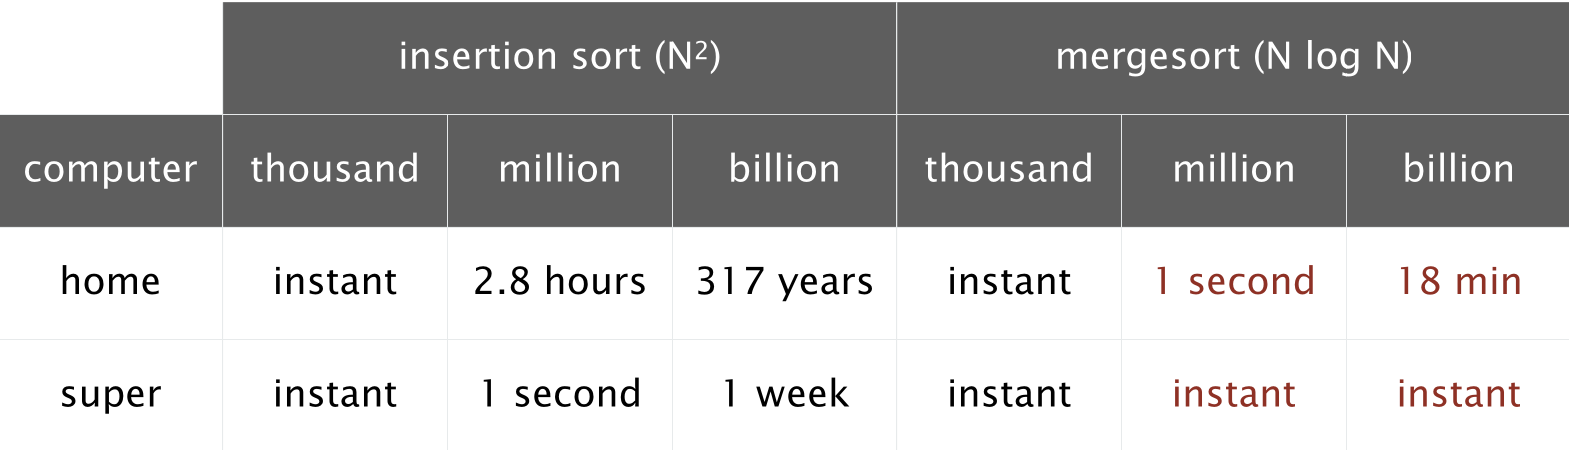
\includegraphics[width=.8\textwidth]{img/compara-insert-merge.png}
			\caption{Tabela de comparação de Insertsort e Mergesort. Fonte: Adaptado de \cite{sedgewick2014algorithms}}.
	  \end{figure}

		Conclusão?\\ \pause
		\tcb{Bons algoritmos são melhores do que supercomputadores}.

	\end{frame}
	% ==========================================

	% ==========================================
	\begin{frame}
		\frametitle{Análise Mergesort Recursivo}
	  \begin{block}{Vantagens}
			\begin{itemize}
				\item Mergesort é \textbf{$O(n \log_{2}{n})$};
				\item Indicado para aplicações que tem restrição de tempo (executa sempre em um determinado tempo para \textbf{$n$});
				\item Passível de ser transformado em estável:
					\begin{itemize}
							\item Tomado certos cuidados na implementação da intercalação.
					\end{itemize}
				\item Fácil implementação.
			\end{itemize}
	  \end{block}
	  \begin{block}{Desvantagens}
			\begin{itemize}
				\item Utiliza memória adicional, em \textbf{$O(n)$}:
					\begin{itemize}
							\item Existem implementações que não necessitam de espaço adicional, mas são complexas;
					\end{itemize}
				\item Na prática é mais lento que \textbf{Quicksort} no caso médio.
			\end{itemize}
	  \end{block}
  \end{frame}
	% ==========================================

	\section{Implementação Iterativa}

	\begin{frame}[c]{Mergesort Iterativa}

		Você consegue implementar a versão iterativa do Mergesort?\\
		Qual a complexidade da sua implementação?

	\end{frame}
	
	\section{Otimizações práticas}

	\begin{frame}[c]{Possíveis otimizações}

		Embora o \textbf{Mergesort} seja considerado como assintoticamente ótimo\footnote[frame]{O número de comparações realizado pelo Mergesort no pior caso é o menor número de comparações possível para qualquer algoritmo de ordenação \textit{baseado em comparações} \cite{sedgewick2014algorithms}.}, algumas otimizações simples podem ser realizadas para deixá-lo ainda mais eficiente. Dentre elas:

		\begin{itemize}
				\item Utilizar Insertsort em partes pequenas do array;
				\item Não realizar a operação merge caso a coleção já esteja ordenada;
				\item Eliminar a cópia para um array auxiliar (poupa tempo mas não espaço);
				\item Aproveitar trechos pré-ordenados;
		\end{itemize}

		Mas lembre-se, embora essas otimizações tornem o algoritmo mais eficiente em alguns casos, sua complexidade ainda é $O(n \log_{2}{n})$ no pior caso.


	\end{frame}

	\begin{frame}[c]{Insertsort para pequenas porções}

		\begin{itemize}
				\item Mergesort tem muito overhead para arrays pequenos;
				\item Determinar uma linha de corte (\textit{cutoff}): trechos com um número menor de elementos do que a linha de corte são ordenados por Insertsort;
		\end{itemize}

	\end{frame}
	\begin{frame}[c]{Insertsort para pequenas porções}

	  \begin{figure}[h]
	  	\centering
	  	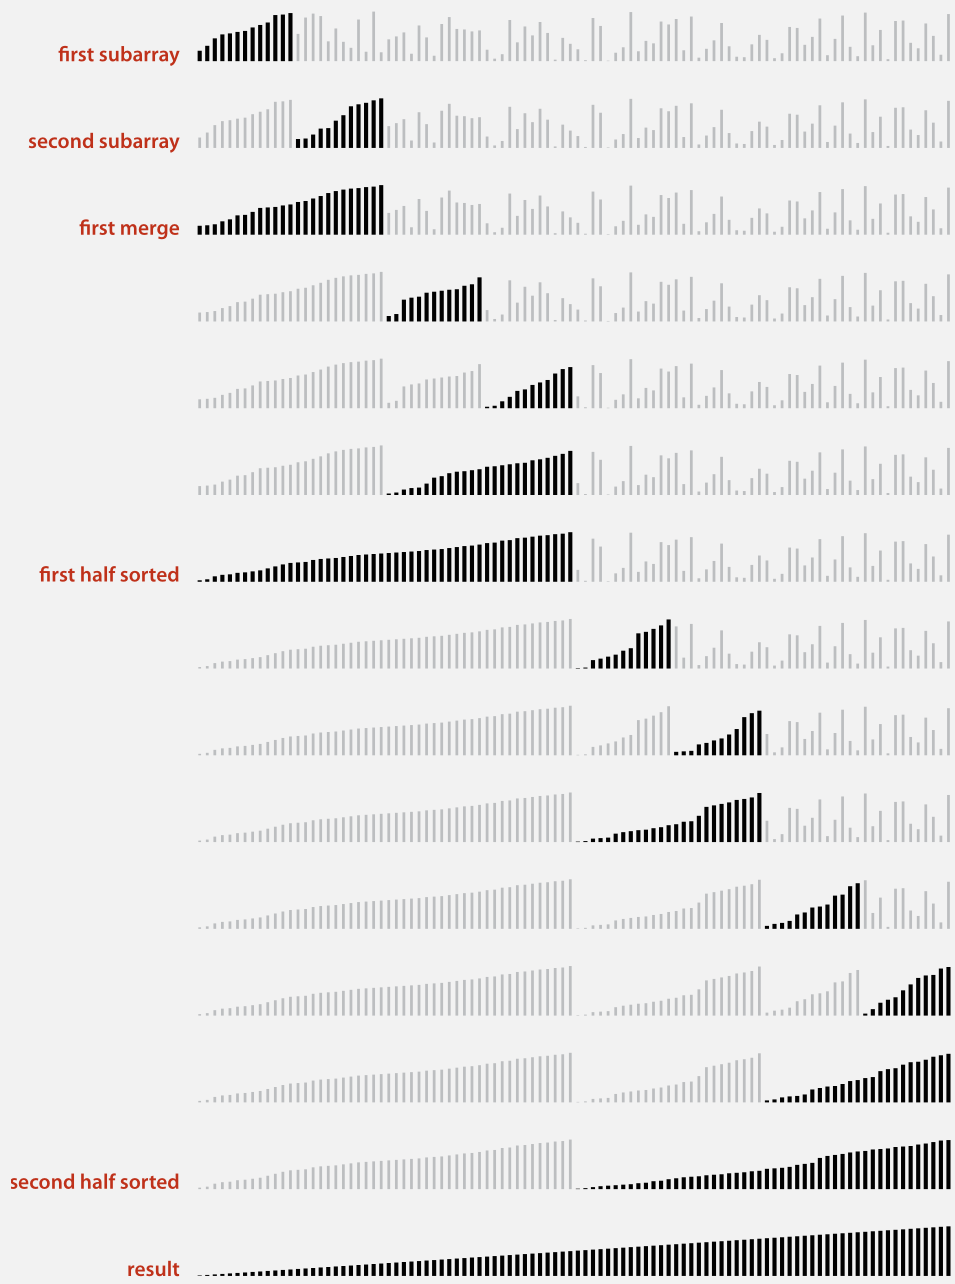
\includegraphics[width=.4\textwidth]{img/insertsort.png}
			\caption{\tiny Mergesort com cutoff para insertion sort. Fonte: \cite{sedgewick2014algorithms}}
	  \end{figure}

	\end{frame}
	\begin{frame}[fragile,c]{Impedir merge caso seja desnecessário}

	  \begin{figure}[h]
	  	\centering
	  	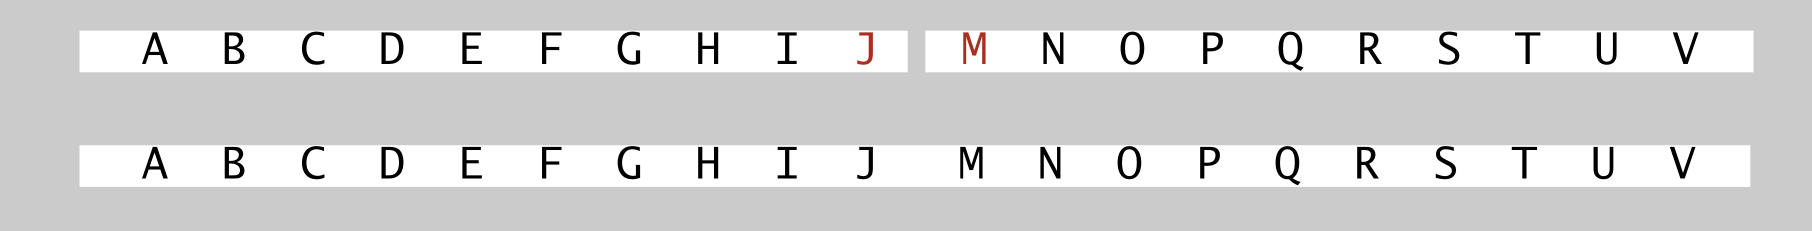
\includegraphics[width=\textwidth]{img/no-merge.png}
			\caption{\tiny Mergesort sem merge desnecessário. Fonte: \cite{sedgewick2014algorithms}}
	  \end{figure}
	
		\begin{minted}[frame=lines,framesep=2mm,baselinestretch=1.2,fontsize=\normalsize,linenos]{c}
	// ...
	mergesort(a, l, m);
	mergesort(a, m+1, r);
	if(a[m] <= a[m+1]) return;
	// ...
		\end{minted}

	\end{frame}

	\begin{frame}[fragile, c]{Mergesort natural}
		\begin{itemize}
				\item Aproveitar trechos já ordenados da coleção:
		\end{itemize}

	  \begin{figure}[h]
	  	\centering
	  	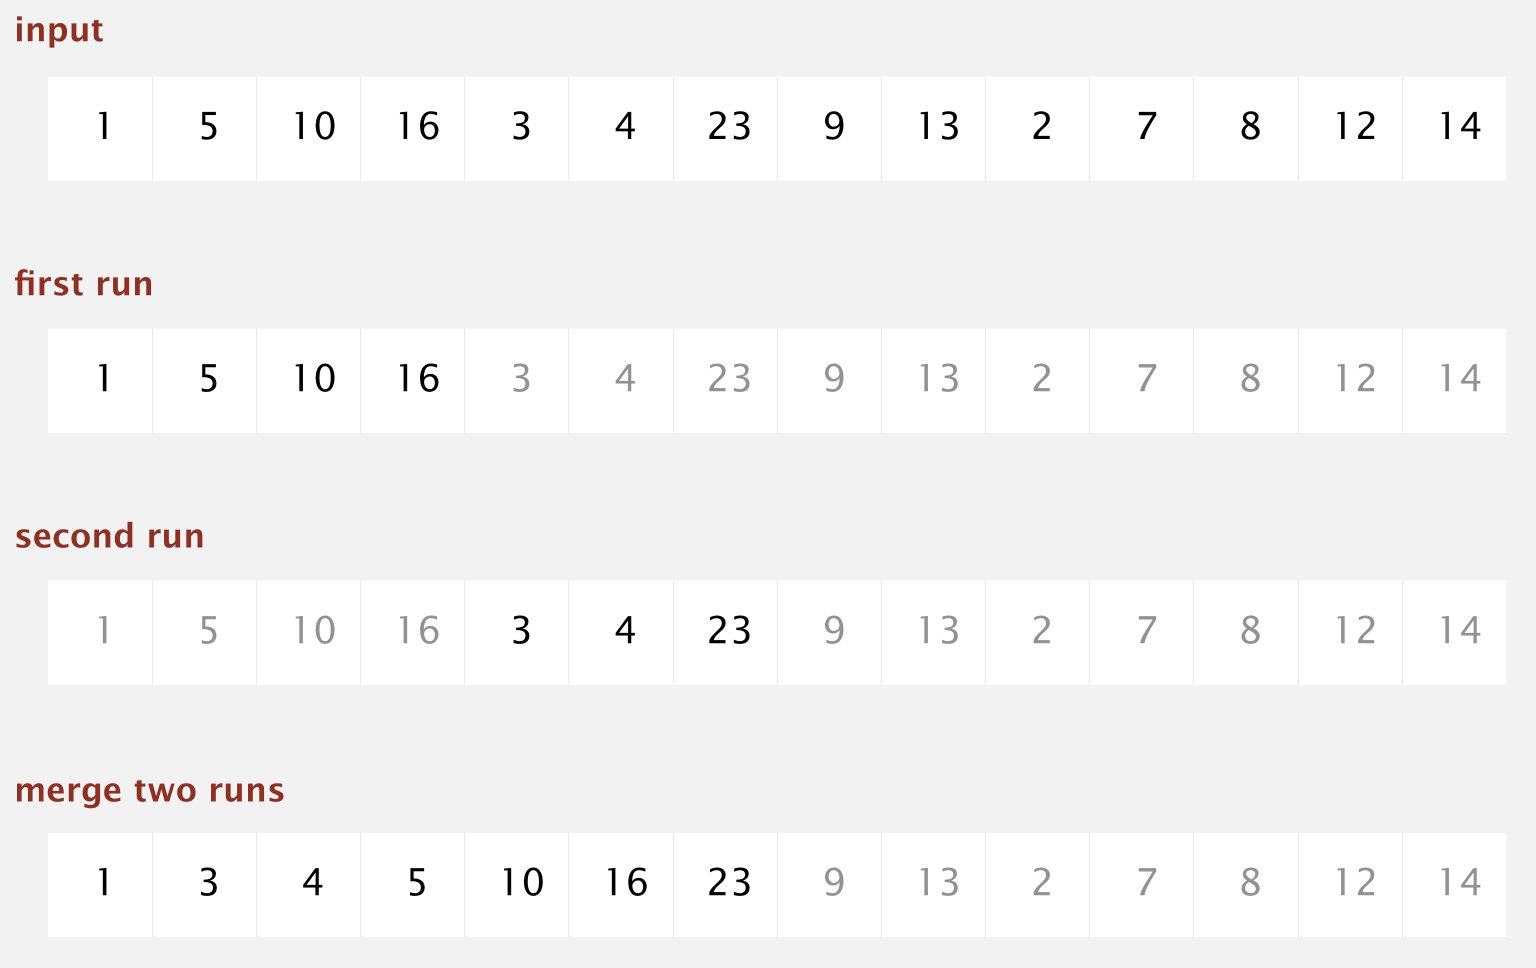
\includegraphics[width=.8\textwidth]{img/merge-natural.png}
			\caption{\tiny Mergesort natural. Fonte: \cite{sedgewick2014algorithms}}
	  \end{figure}

	\end{frame}

	\begin{frame}[fragile, c]{Eliminar cópia para array auxiliar}

		\begin{itemize}
				\item Executar a cópia apenas uma vez, antes da ordenação;
				\item Para cada chamada recursiva, alternar o papel entre o array original e o auxiliar:
		\end{itemize}
		
		\begin{minted}[frame=lines,framesep=2mm,baselinestretch=1.2,fontsize=\small,linenos]{c}
void mergesort(int * a, int * aux, int l, int r){
	// ...
	mergesort(aux, a, l, m);    // <- aux e a inverteram de posição
	mergesort(aux, a, m+1, r);  // <- aux e a inverteram de posição
	// ...
}
		\end{minted}

		\begin{itemize}
				\item Economiza tempo, mas não espaço, uma vez que ainda precisamos de um array adicional.
		\end{itemize}
	\end{frame}

	
	\section{Conclusão}
	
	% ==========================================
	\begin{frame}
		\frametitle{Algoritmos de ordenação}
	  \begin{figure}[h]
	  	\centering
	  	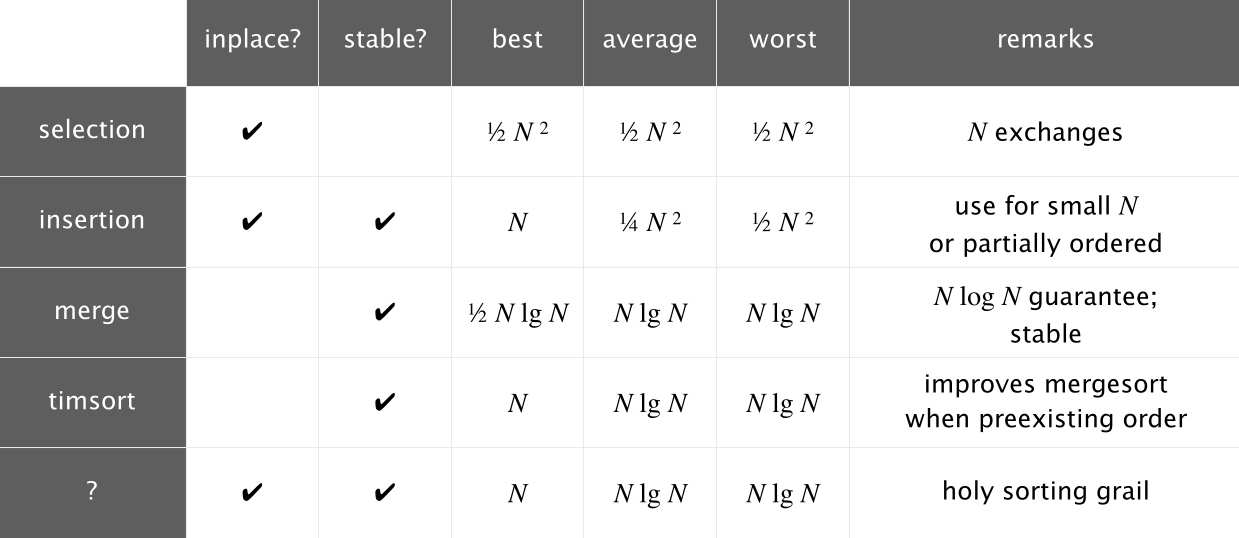
\includegraphics[width=\textwidth]{img/table.png}
			\caption{\footnotesize Tabela de comparação de algoritmos de ordenação. Fonte: Adaptado de \cite{sedgewick2014algorithms}}
	  \end{figure}
		
		\small Curiosidade: algoritmo chamado \tcb{Timsort} (que é a implementação de algumas das otimizações apresentadas) é o algoritmo utilizado em algumas bibliotecas padrão de linguagens e ambientes como: Python, Java 7, GNU Octave, Android, ...
	\end{frame}
	% ==========================================

	\begin{frame}[c]{Conclusão}

		\begin{itemize}
			\item Algoritmo assintoticamente ótimo para o problema da ordenação geral;
			\item Fácil implementação;
			\item Otimizações práticas;
		\end{itemize}

	\end{frame}
	
	\section{Prática}

	\begin{frame}[c]{Exercícios sugeridos}
Além de implementar a versão iterativa do Mergesort, realize os seguinte exercício para fixação do algoritmo:
		\begin{itemize}
			\item Dada a sequencia de números: $[3, 4, 9, 2, 5, 1, 8]$, ordene em ordem crescente utilizando o algoritmo Mergesort passo-a-passo (teste de mesa).
		\end{itemize}

	\end{frame}

	% ==========================================
	% \begin{frame}[fragile,c]{Implementação Recursiva Fatorial}
	%	\begin{minted}[frame=lines,framesep=2mm,baselinestretch=1.2,fontsize=\normalsize,linenos]{c}
	%	\end{minted}
	% \end{frame}
	% ==========================================

	% ==========================================
	% \begin{frame}
	% 	\frametitle{Título}
	% 	\begin{itemize}
	% 		\item Item bla bla bla
	% 	\end{itemize}
	%	  \begin{block}{Título de bloco}
	%		 	Conteúdo do bloco
	%   \end{block}
	% \end{frame}
	% ==========================================

	% ==========================================
	% Exemplo de frame com figura
	% \begin{frame}
	% 	\frametitle{Título}
	%	  \begin{figure}[h]
	%	  	\centering
	%	  	\includegraphics[width=10cm]{paht.png}
	%			\caption{Bla bla bla ...}
	%	  	\label{label}
	%	  \end{figure}
	% \end{frame}
	% ==========================================

	% ==========================================
	% Exemplo de frame com algoritmo
	% \begin{frame}[fragile]
	% 	\frametitle{Título}
	% 	\begin{lstlisting}[language=C]
	% 		#include <stdio.h>
	%
	% 		int main()
	% 		{
	% 		  int a[5];
	%
	% 		  a[0] = 30;
	% 		  a[1] = 25;
	% 		  a[2] = 5;
	% 		  a[3] = 100;
	% 		  a[4] = 1;
	%
	% 		  printf("%d\n",a[1]);
	% 		}
	% 	\end{lstlisting}
	% \end{frame}
	% ==========================================

	% ==========================================
	% Frame para referências
	\begin{frame}[allowframebreaks]
		\frametitle{Referências utilizadas na apresentação}
		\bibliography{referencias}
	\end{frame}
  % ==========================================

\end{document}
